
\documentclass[11pt]{article}
\usepackage[review]{nlp4call} 
%\usepackage[final]{nlp4call}
\usepackage{times}
\usepackage{xurl}
\usepackage{url}
\usepackage{latexsym}
\usepackage{amsmath}
\usepackage{amssymb}
\usepackage{graphbox}
\usepackage{graphicx}
\usepackage{hyperref}
\usepackage{tabularx}
\usepackage{tikz}
\usepackage{titling}
\usepackage{makecell}
\usepackage{float}
\usepackage[ruled,linesnumbered]{algorithm2e}
\usepackage{algpseudocode}
\usepackage{listings}
\usepackage{xcolor}

\graphicspath{{../images/}}

\definecolor{codegreen}{rgb}{0,0.6,0}
\definecolor{codegray}{rgb}{0.5,0.5,0.5}
\definecolor{codepurple}{rgb}{0.58,0,0.82}
\definecolor{backcolour}{rgb}{0.95,0.95,0.92}

\lstdefinestyle{mystyle}{
    backgroundcolor=\color{backcolour},   
    commentstyle=\color{codegreen},
    keywordstyle=\color{magenta},
    numberstyle=\tiny\color{codegray},
    stringstyle=\color{codepurple},
    basicstyle=\ttfamily\footnotesize,
    breakatwhitespace=false,         
    breaklines=true,                 
    captionpos=b,                    
    keepspaces=true,                 
    numbers=left,                    
    numbersep=5pt,                  
    showspaces=false,                
    showstringspaces=false,
    showtabs=false,                  
    tabsize=2
}

\lstset{style=mystyle}

\title{Algorithmic Analysis of Graph Isomorphism}
\author{maximum-solution}
\date{}

\begin{document}
\nolinenumbers
\maketitle
\begin{abstract}
  This document contains an algorithmic analysis of a computational problem i.e. graph isomorphism. The problem is also called "graph matching" problem and lies at the heart of myriad fields including computer vision and pattern recognition. Such an importance drives need to look for solutions that are not only appropriate but also efficient. The objective of this paper is to analyse time efficiency of solving graph isomorphism problem using different algorithmic design techniques.   
\end{abstract}

\section{Introduction}

Our project focuses on the graph isomorphism problem. It is computational problem of finding if two graphs are isomorphic. Our project will also talk about which approach is optimal to solve this problem. Graph isomorphism remains one of the most important and efficiently unresolved problems and it is an NP-complete problem. this problem has been studied since the early days of computing. On the theoretical side, this problem focuses on algorithmic group theory and it has many application domains. Graph isomorphism gained importance in the 1970s, it came as a natural problem in the complexity of NP class (NP-complete) and cannot be solved in polynomial time. This problem comes in the area of pattern matching and we chose this problem because it is used in many applications, for example, image processing, protein structure, chemical bond structure, and Social Networks (more details about its applications are given in the Application section). Graph Isomorphism is an NP-intermediate problem as all the current solutions are not in polynomial time. In this paper, we are going to explain a couple of design techniques that will determine whether two graphs are isomorphic, their vertices and edges are the same, and their connectivity is retained, and we will tell which design techniques are optimal to find isomorphic between two graphs.\\

\section{Overview of Technique}

We have presented three solutions for the graph isomorphism problem including a brute force approach, divide \& conquer approach and Weisfeiler-Lehman algorithm (WL). Our strategy for the algorithmic analysis proceeds by first defining the design pattern and approach of each algorithm. Then proposing pseudo-code for the algorithm. Stating the implementation details and testing of the algorithm. Finally conducting run-time complexity analysis of the algorithm. The procedure will be repeated for all three proposed solutions in isolation. Once we have conducted individual analysis, then we will take a holistic approach. A small scale comparative analysis would be conducted for the three solutions to clearly observe that how algorithmic designs can have significant impact on time complexity and hence efficiency of the problem. Our hypothesis for the results is that brute force will provide most inefficient response, Divide and conquer would be better than brute force and WL algorithm will be better among the three. However, we doubt if any of these solutions would result in a true polynomial run-time complexity as mentioned before, graph isomorphism is a problem that is known to lie between NP and P so far. 
\section{Overview of Testing}
The three algorithms will be tested on the same test data. All three algorithms takes two adjacency matrix representation of an undirected - unweighted graphs as input and returns a Boolean output i.e. True if the two graphs are isomorphic otherwise False. For the brute force algorithm, since the run-time complexity is very high, we were not able to test it for quantitatively large data (graph with larger number of vertices and edges) due to limited processing power of the machine however we have attempted to test it for fairly large input. \\
The test data has been generated, using a helper function, named, generate\_random\_graph(n), it takes parameter n which represents the number of nodes in the graph.
\section{Algorithm I: \textit{Brute Force}}
The section presents a naive-trivial algorithm to solve graph isomorphism \cite{bruteGI} problem.It is important to mention that the presented is highly inefficient.
\subsection{Approach}
We know that two graphs are isomorphic if they are structurally equivalent. This structural equivalency indicates similar vertex-edge pattern. In the brute force algorithm, our goal will be to make use of the definition of graph isomorphism. Our design can be divided up into three basic tests:\\
\textbf{Test 1:}\\
In the first step, we will check if the two input graphs have the same graph order. By graph order, we means the number of vertices. The algorithm will proceed to the next test only if two input graphs are such that they have the same number of vertices otherwise it would be concluded that he two graphs are not isomorphic. Graph orders has been achieved by a helper function named \textit{get\_graph\_order()} \\
\textbf{Test 2};\\
Since, we have established in the previous test that the two graphs have the same number of vertices, now we will check for the degree sequence. By degree sequence we mean a list of degree i.e. the number of edges incident with it, usually sorted in a non increasing order. If the degree sequence of the two input graphs is equal only then algorithm will proceed to the nest test otherwise it would be concluded that graphs are not isomorphic. Degree sequence has been achieved by a helper function named \textit{get\_degree\_sequence()} \\\\
\textbf{Test 3};\\
Finally if the two previous test passes, we will select any one of the two input graph and generate all possible permutations of its vertices. Each permutation will be compared with the other input graph and if anyone permutation matches, then we can conclude that the graphs are isomorphic otherwise not. It is the most expensive component of this algorithm as we are generating all possible permutations that might be trivial for the small number of vertices but will increase be drastically complicated for large graphs. All vertex permutation has been achieved by a helper function named \textit{get\_all\_vertex\_permutations} \\
The pseudo-code for this approach can be found in the next section. 
\label{sect:pdf}
\subsection{Pseudo-Code}
\SetAlgoLined
\begin{algorithm}
  \DontPrintSemicolon
  \KwData{Graph adjacency matrix, $adj_1$, $adj_2$}
  \KwResult{Whether graphs are isomorphic or not, bool.}
  
  $degree\_sequence\_1 \gets get\_degree\_sequence(adj_1)$\;
  $degree\_sequence\_2 \gets get\_degree\_sequence(adj_2)$\;
  \If{$get\_graph\_order(adj_1)$ != $get\_graph\_order(adj_2)$}{\Return False}
  \Else{
  \If{$degree\_sequence\_1$ != $degree\_sequence\_2$}{\Return False}
  }
  \Else{
  \For{$adj\_mat$ in $get\_all\_vertex\_permutations(adj_2))$}
  {
  \If{$adj\_mat$ == $adj_1$}{\Return True}
  }
  }
  \Return False
  \caption{Brute-Force GI}
  \label{algorithm1}
\end{algorithm}

\begin{algorithm}
  \DontPrintSemicolon
  \KwData{Graph adjacency matrix, $adj\_mat$}
  \KwResult{Number of Vertices, integer.}
  \If{$len(adj\_mat)$ != $len(adj\_mat[0])$}{\Return\ -1}
  \Else{
    \Return $len(adj\_mat)$
  }
  \caption{Helper Function: get\_graph\_order()}
\end{algorithm}

\begin{algorithm}
  \DontPrintSemicolon
  \KwData{Graph adjacency matrix, $adj\_mat$}
  \KwResult{Number of Vertices, integer.}
  $degree\_sequence \gets []$\;
  \For{$i = 0$ \textbf{to} $len(adj\_mat)$}
  {
  $degree\_sequence.append (sum(adj\_mat[i]))$\;
  $degree\_sequence$.sort(reverse=True)\;
    \Return $degree\_sequence$
  }
  \caption{Helper Function: get\_degree\_sequence()}
\end{algorithm}

\begin{algorithm}
  \DontPrintSemicolon
  \KwData{Graph adjacency matrix, $adj\_mat$}
  \KwResult{list of all adjacency matrices, list.}
  $all\_adj\_matrix \gets []$\;
  $idx = range(len(adj_matrix))$\;
  $possible\_idx\_combinations \gets permutations(idx, len(idx)$\;
 \For{$idx\_comb$ in $possible\_idx\_combinations$}
  {
  $a = transpose(transpose(a)[idx_comb])$\;
  $all\_adj\_matrix.append(a)$\;
  }
   \Return $all\_adj\_matrix$
  \caption{Helper Function: get\_all\_vertex\_permutations}
\end{algorithm}
\subsection{Implementation Details}
\label{ssec:layout}
We have implemented the above pseudo-code in python. The adjacency matrix representation of graph has been achieved using 2D array. We have implemented it in a function named \textit{brute\_force\_test\_graph\_isomorphism}\\
\begin{lstlisting}[language=Python]
def brute_force_test_graph_isomporphism(adj_1, adj_2):
    degree_sequence_1 = get_degree_sequence(adj_1)
    degree_sequence_2 = get_degree_sequence(adj_2)
    if get_graph_order(adj_1) != get_graph_order(adj_2):
        return False
    elif np.array_equal(degree_sequence_1, degree_sequence_2) == False:
        return False
    else:
        for adj_matrix in list(
                map(lambda matrix: matrix["adj_matrix"],
                    get_all_vertex_permutations(adj_2))):
            if np.array_equal(adj_1, adj_matrix) == True:
                return True
    return False
\end{lstlisting}
The implementation of helper function to find graph order is as follows:
\begin{lstlisting}[language=Python]
def get_graph_order(adj_matrix):
    if len(adj_matrix) != len(adj_matrix[0]):
        return -1
    else:
        return len(adj_matrix)
\end{lstlisting}
The implementation of helper function to find degree sequence is as follows:
\begin{lstlisting}[language=Python]
def get_degree_sequence(adj_matrix):
    degree_sequence = []
    for vertex in range(len(adj_matrix)):
        degree_sequence.append(sum(adj_matrix[vertex]))
    degree_sequence.sort(reverse=True)
    return degree_sequence
\end{lstlisting}
The implementation of helper function to find all permutations of vertices is as follows:
\begin{lstlisting}[language=Python]
def get_all_vertex_permutations(adj_matrix):
    all_adj_matrix = []
    idx = list(range(len(adj_matrix)))
    possible_idx_combinations = [
        list(i) for i in itertools.permutations(idx, len(idx))
    ]
    for idx_comb in possible_idx_combinations:
        a = adj_matrix
        a = a[idx_comb]
        a = np.transpose(np.transpose(a)[idx_comb])
        all_adj_matrix.append({
            "perm_vertex":
            idx_comb,
            "adj_matrix":
            a
        })

    return all_adj_matrix
\end{lstlisting}
\subsection{Testing Details}
\label{ssec:fonts}
The above python implementation of brute force algorithm was tested on randomly generated undirected-unweighted graphs. We wish to test on larger number of vertices however due to an inefficient performance of the algorithm and limited processing power of machine, the algorithm was successfully tested up to graph with 14 vertices only. The test data can be found in git repository at demo $\rightarrow$ input\\ We also conducted an experimental complexity analysis of the implementation. The strategy used for the purpose was that the algorithm was run on graph with vertices (n) = 2 to n=14 and time was recorded using the python time module, \textit{timeit}. We repeated experiment five times for every graph and then calculated the average run-time for each n. 

\subsection{Results}
\label{ssec:first}
The result of our experimental analysis are summarized in the following plot:
\begin{center}
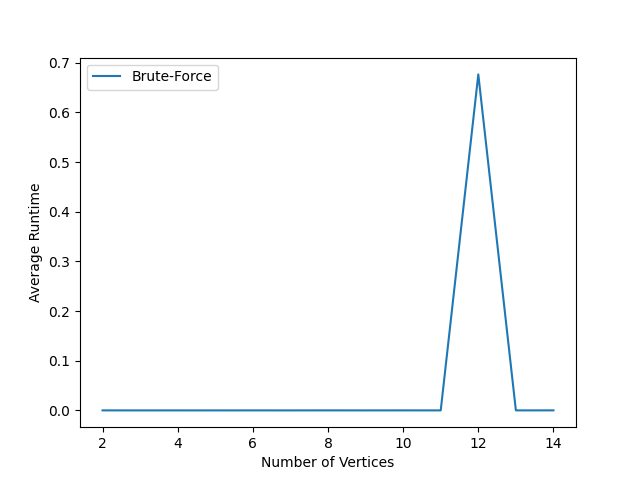
\includegraphics[width=7cm]{brute_plot.png}\\
\end{center}
As it can be noticed from the plot above that higher number of vertices, the slope of the plot is large. Even though the O(n!) trend is not quite visible from the plot as our machine allowed execution up to a small number of n only and a clearer picture would have achieved if the algorithm could be tested for wider range of n, however we can predict from the steep plot and large enough rate of increase for n=14, that the for the graph with larger n, execution plot would increase with faster rates.


\section{Algorithm II: \textit{VF2 Algorithm}}
In this section, an implementation of VF2 algorithm is discussed. Isomorphism is a mapping, $M$, between two graphs, $G_1$ and $G_2$ in which $M$ maps each branch of $G_1$ to branch in $G_2$ and vice versa \cite{cordella2001improved}. The implicit design technique for this algorithm is divide and conquer.   

\subsection{Approach}
Let's consider two graphs, $G_1$ and $G_2$ that needs to be matched. There is a mapping function, $M$, $M(s)$ contains the subset of this function. Here, $s$ is a state of partial mapping and $M(s)$ is a partial mapping solution. This partial mapping is basically an identification of subgraphs in $G_1$ and $G_2$ at a specific state $s$ and it only includes the nodes and the branches connecting them. Some important terminologies are listed below:
\begin{enumerate}
    \item $M_1(s)$: The projection of $M_1(s)$ onto set of nodes, $N_1$, of $G_1$.
    \item $M_2(s)$: The projection of $M(s)$ onto set of nodes, $N_2$, of $G_2$.
    \item $B_1(s):$ Set of branches of $G_1$. 
    \item $B_2(s):$ Set of branches of $G_2$.
    \item Pred($G, n$)(the predecessors of $n$): Set of nodes $G$ from which a branch originates till $n$. 
    \item Succ($G, n$)(the successors of $n$): Set of nodes $G$ branching from $n$.
    \item $T^{\text{out}}_1(s)(out-terminal):$ Set of nodes of $G_1$ that are successors of $M_1(s)$ nodes and are not part of $M_1(s)$ nodes.
    \item $T^{\text{out}}_2(s)(out-terminal):$ Set of nodes of $G_2$ that are successors of $M_2(s)$ nodes and are not part of $M_2(s)$ nodes.
    \item $T^{\text{in}}_1(s)(in-terminal):$ Set of nodes of $G_1$ that are predecessors of $M_1(s)$ nodes and are not part of $M_1(s)$ nodes.
    \item $T^{\text{in}}_1(s)(in-terminal):$ Set of nodes of $G_2$ that are predecessors of $M_2(s)$ nodes and are not part of $M_2(s)$ nodes.
\end{enumerate}

The specific parts of the algorithm are described below:
\subsubsection{Defining set $P(s)$}
If both $T^{\text{out}}_1(s)$ and $T^{\text{out}}_2(s)$ are not empty then $P(s)$ can be defined as:
\[ P(s) = T^{\text{out}}_1(s) \times \{ \text{min} T^{\text{out}}_2(s) \} \]
Here the min refers to the node having the smallest label. Now, if both $T^{\text{out}}_1(s)$ and $T^{\text{out}}_2(s)$ are empty, and both $T^{\text{in}}_1(s)$ and $T^{\text{in}}_2(s)$ are not, then
\[ P(s) = T^{\text{in}}_1(s) \times \{ \text{min} T^{\text{min}}_2(s) \} \]
Now, if all four are empty, then
\[ P(s) = (N_1 - M_1(s) \times \{ \text{min} (N_2 - M_2(s)) \} \]
Where $N_1$ and $N_2$ are set of nodes for $G_1$ and $G_2$ respectively. The whole idea of $P(s)$ is to make sure that the algorithm does not visit the same state again. This is achieved by declaring a state $s$ is not part of a matching when only one of the in-terminal sets or out-terminal sets is empty. Then the state $s$ is not explored anymore.
\subsubsection{Feasibility Function (F(s, n, m)}
In this function, all the nodes connected to $n$ and $m$ are examined. If they exist in current partial mapping, then each branch from or to $n$ is checked for mapping with each branch from or to $m$. Otherwise, the algorithm will check the number of nodes in $T^{\text{in}}_i(s), T^{\text{out}}_i$ and $(N_i - M_i(s) - T_i^{\text{in}} - T_i^{\text{out}}(s))$ and for isomorphism to exist, these counts should be equal for $n$ and $m$. For this mapping, it is important that it holds the compatibility which depends on the application.

\subsubsection{Data Structures Used}
\begin{enumerate}
    \item Two vectors with dimensions same as number of nodes in $G_1$ and $G_2$ containing the current mapping. 
    \item Four vectors to describe the membership of terminal sets and whose dimensions are equal to the number of nodes of corresponding graphs.
\end{enumerate}

\subsubsection{Summary}
This algorithm can be used for both sub-graph isomorphism and graph isomorphism. This algorithm makes use of the semantic information of nodes and branches. VF2 is a divide and conquer algorithm to find if two graphs are isomorphic. The main idea is to create a state s that contains a partial mapping between nodes of G1 and G2. M(s) identifies the two sub graphs and includes nodes and branches. Here s is the state of mapping. Now, M(s) is extended and new branches are included with pair (n, m) where n and m nodes belongs to each graph. Through certain feasibility rules, consistent states are maintained(1). Moreover, in terms of space complexity, the algorithm has a small memory requirement which makes it suitable for large graphs.

\label{sect:pdf}
\subsection{Pseudo-Code}
\begin{algorithm}
  \DontPrintSemicolon
  \KwData{Intermediate state $s$; the initial state $s_0$ has $M(s_0) = null$}
  \KwResult{Mapping between two graphs.}
  \If{$M(s)$ covers all the nodes of $G_2$}{\Return $M(s)$}
  \Else{compute the set $P(s)$ of the pairs candidate for inclusion in $M(s)$\;
  \For{$(n, m) \in P(s)$}{
    \If{$F(s, n, m)$}{compute the state $s$ obtained by adding $(n, m)$ to $M(s)$\; Match($s$)}}}
  \caption{Match function of VF2 Algorithm}
\end{algorithm}

\subsection{Implementation Details}
\label{ssec:layout}
This algorithm is available as part of networkx library \cite{bruteGI} to be implemented in Python. We used input as an adjacency list and converted it to graph in networkx library. 
\begin{lstlisting}[language=Python]
import networkx.algorithms.isomorphism as iso
import networkx as nx

def VF2(G1, G2):
    Graph_Matcher = nx.isomorphism.GraphMatcher(G1, G2)
    return Graph_Matcher.is_isomorphic()
\end{lstlisting}
Here, the Graph Matcher class matches the graphs in predetermined manner. Here, the feasibility function is utilized. The feasibility function is either semantic or syntactic. The isomorphism function of the class is as follows:
\begin{lstlisting}[language=Python]
def is_isomorphic(self):
    """Returns True if G1 and G2 are isomorphic graphs."""

    # Check global properties
    if self.G1.order() != self.G2.order():
        return False

    # Check local properties
    d1 = sorted(d for n, d in self.G1.degree())
    d2 = sorted(d for n, d in self.G2.degree())
    if d1 != d2:
        return False

    try:
        x = next(self.isomorphisms_iter())
        return True
    except StopIteration:
        return False
\end{lstlisting}
The match function (main function) is as follows:
\begin{lstlisting}[language=Python]
def match(self):
    """Extends the isomorphism mapping.

    This function is called recursively to determine if a complete
    isomorphism can be found between G1 and G2.  It cleans up the class
    variables after each recursive call. If an isomorphism is found,
    we yield the mapping.

    """
    if len(self.core_1) == len(self.G2):
        # Save the final mapping, otherwise garbage collection deletes it.
        self.mapping = self.core_1.copy()
        # The mapping is complete.
        yield self.mapping
    else:
        for G1_node, G2_node in self.candidate_pairs_iter():
            if self.syntactic_feasibility(G1_node, G2_node):
                if self.semantic_feasibility(G1_node, G2_node):
                    # Recursive call, adding the feasible state.
                    newstate = self.state.__class__(self, G1_node, G2_node)
                    yield from self.match()

                    # restore data structures
                    newstate.restore()
\end{lstlisting}

\subsection{Testing Details}
\label{ssec:fonts}
The algorithm worked perfectly fine up to the size of 40 inputs. timeit library was used to test the time duration. The input were files that were converted to networkx graphs and on them the algorithm was applied. All the test data is available in git repository. 

\subsection{Results}
\begin{figure}[H]
    \centering
    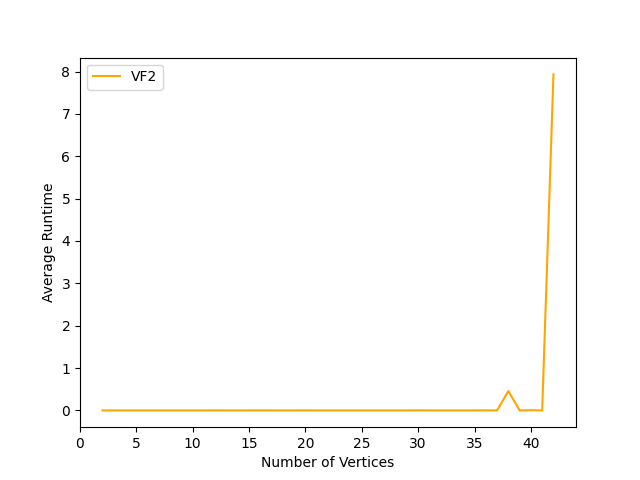
\includegraphics[width=7cm]{vf2.png}
\end{figure}
\label{ssec:first}


\section{Algorithm III: \textit{Weisfeiler–Lehman (WL) Algorithm}}

\subsection{Approach}
Weisfeiler-Lehman Algorithm \cite{shervashidze2011weisfeiler} tests for graph isomorphism based on color refinement and is a randomized algorithm. Let the two graphs to be tested for isomorphism be $G_1 = (V_1, E_1)$ and $G_2 = (V_2 , E_2)$ where $|V_1| = |V_2|$ and $|E_1| = |E_2|$.\\
Initially, all the vertices of $G_1$ and $G_2$ are assigned a same color where a color can be represented by an integer.For each vertex in $G_1$, a set with repetitions i.e. a multi-set of the colors of its neighbors is created. Same is done for $G_2$. Next, the vertices that held same color and multi-set pair previously are only recolored so that so that the two vertices have the same color. If the two multi-sets hold identical color pairs then the graphs are said to be isomorphic. However, there is a possibility for two non-isomorphic graphs to share identical multi-sets. To mitigate this, the above approach can be iterated $k$ which is known as \textit{k-dimensional Weisfeiler Lehman Algorithm}. In the \textit{k-dimensional} version of this algorithm, we color \textit{k-tuples} of vertices where there exists \textit{k} such that \textit{k-WL} identifies all planar graphs \cite{grohe2017color}. 3-dimensional WL algorithm is known to accurately distinguish  all planar graphs \cite{wlTest}, hence, in our implementation we have set $k = 3$.

\label{sect:pdf}
\subsection{Pseudo-Code}
\begin{algorithm}
  \DontPrintSemicolon
  \KwData{Two graphs to be tested for isomorphism, $G_1$ and $G_2$}
  \KwResult{True if graphs are isomorphic else False}
  G1Neighbors = getNeighbors(G1)\;
  G2Neighbors = getNeighbors(G2)\;
  Assign initial Color $c_0$ to each $v \in G_1$\;
  Assign initial Color $c_0$ to each $v \in G_1$\;
  \For{i $\in$ (0,kdim)}{
      \For{$v \in V_1$}{
      Store collection of colors of neighbours of $v$\;}
      \For{$v \in V_1$}{
      Store collection of colors of neighbours of $v$\;}
      Prepare color - collection pairs $(c , l)$ for each vertex in $G_1$ and $G_2$\;
      Assign new color to each vertex in $G_1$ and $G_2$\;
      }
    \If{colors of $v_i$ == colors of $u_i$}{\Return true}
\Else{\Return False}
  \caption{Match function of WL Algorithm}
\end{algorithm}
\subsection{Implementation Details}
The above pseudocode was implemented in python and adapted from \cite{wlTest}
\label{ssec:layout}
\begin{lstlisting}[language=Python]
import bisect

def neighbour_list(matrix):
    result = []
    n = len(matrix)
    for i in range(n):
        result.append([])
    for i in range(n - 1):
        for j in range(i, n):
            if matrix[i][j]:
                result[i].append(j)
                result[j].append(i)
    return result





def wl_method(graph1, graph2):
        graph_1_neighbour_list = neighbour_list(graph1)
        graph_2_neighbour_list = neighbour_list(graph2)

        n=len(graph1)

        graph_1_colors = [0] * n
        graph_2_colors = [0] * n

        # repeat method method_dim times
        for i in range(1):
            # calc collections of neighbours' colors for each vertex
            graph_1_collection = []
            graph_2_collection = []
            for vertex in range(n):
                neighbours_colors = []
                for neighbour in graph_1_neighbour_list[vertex]:
                    bisect.insort(neighbours_colors, graph_1_colors[neighbour])
                graph_1_collection.append(neighbours_colors)
                neighbours_colors = []
                for neighbour in graph_2_neighbour_list[vertex]:
                    bisect.insort(neighbours_colors, graph_2_colors[neighbour])
                graph_2_collection.append(neighbours_colors)

            # prepare color - collection pairs
            pairs = []
            color_index = 0
            for vertex in range(n):
                collection = graph_1_collection[vertex]
                if not collection in [row[1] for row in pairs]:
                    pairs.append([color_index, collection])
                    color_index += 1

            # check if all collections from graph_2 are in prepared pairs
            for vertex in range(n):
                if not graph_2_collection[vertex] in [row[1] for row in pairs]:
                    return False

            # assign new colors
            for vertex in range(n):
                graph_1_colors[vertex] = pairs[[row[1] for row in pairs].index(graph_1_collection[vertex])][0]
                graph_2_colors[vertex] = pairs[[row[1] for row in pairs].index(graph_2_collection[vertex])][0]

        # on the end compare vertices' colors
        for vertex in range(n):
            if graph_1_colors[vertex] != graph_1_colors[vertex]:
                return False

        # not returned False before
        return True
\end{lstlisting}
\subsection{Testing Details}
\label{ssec:fonts}
The above algorithm was tested on randomly generated graphs with number of vertices $n=2$ till $n=40$. The algorithm was able to produce results identifying isomorphic and non-isomorphic graphs. 
\subsection{Results}
In the plot below, we observe that the execution time increases as the number of vertices increase. 
\label{ssec:first}
\begin{center}
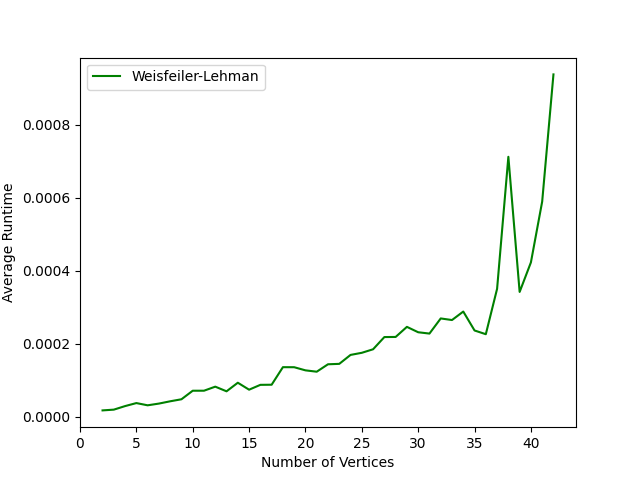
\includegraphics[width=7cm]{wl.png}
\end{center}
\section{Comparative Analysis\cite{tolley1995graph}}
\label{sec:length}
To get a clear picture of run-time efficiency for the aforementioned three graph isomorphism problem solutions, we have performed a comparative run-time analysis for the three algorithms that adds to the individual run-time analysis done in Results section of each algorithm. 
The run-time complexities for the aforementioned three algorithms have been summarized in the table below:
 \begin{figure}[H]
     \centering
     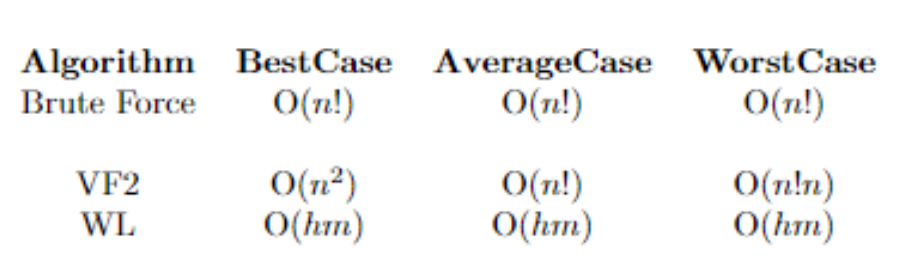
\includegraphics[width=7cm]{table.PNG}
 \end{figure}

We conducted an experimental analysis for the three algorithms in python using \textit{timeit} module. \\
We have run each algorithm on our test data up to n=14 (unfortunately had to select a smaller n due as brute force was irresponsive on larger n due to the limited processing power of machine on which this experiment has been conducted). Each experiment was repeated 5 times to calculated average run-time. The results have been summarized in the plot below:\\
\begin{center}
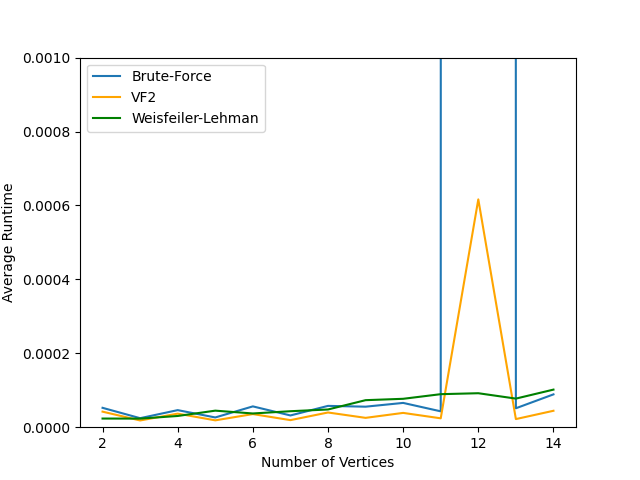
\includegraphics[width=7cm]{experimental.png}
\end{center}
As it can be observed from the plot that brute force tends to perform the worst while WL algorithm better than the other two. However since the number of vertices (n) are very small, we conducted another experiment with comparatively larger number of n, in which only behaviour of WL and VF2 were observed since brute force was not responsive on our machines for larger n. The procedure was same i.e. repeated the experiment 5 times and took average of the run-time.  Following plot summarizes the results:
\begin{center}
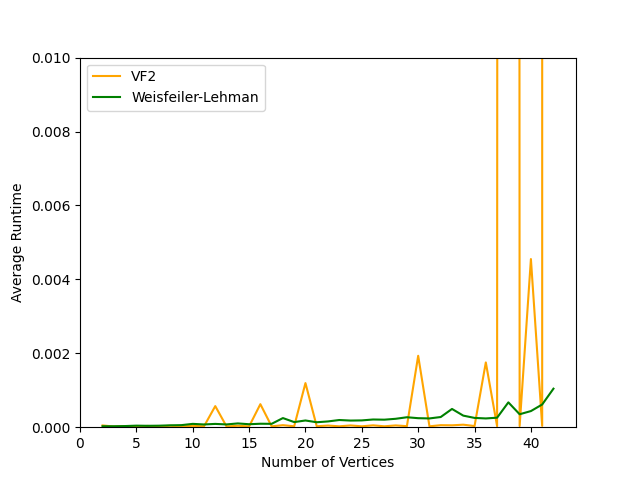
\includegraphics[width=7cm]{exp2.png}
\end{center}
As can be noticed that our observations in the previous experiment about WL were right and it tend to perform better than VF2 for larger values of n too.  All in all our experimental analysis concluded accuracy of our theoretical analysis for the run-time complexity of three algorithms. \\

    It can be established that WL (1D) algorithm would be an appropriate choice for graph isomorphism solution as it has O(hm) run-time complexity when used with the radix sort, where m is the number of elements in multi sets and h is the number of iterations (see WL section for more details on how algorithm works). However, this upper bound seems linear but is actually pseudo-polynomial and depends upon m and h.
    

\section{Can we do Better?}
The answer is \textbf{Yes}. Even though WL provides us with a pseudo-polynomial best case run-time, however it would be better if we can solve the graph isomorphism problem in true polynomial time. One such attempt has been done by Ashay Dharwadker and John-Tagore Tevet and it would not be wrong to suggest that they succeeded. We presents in this section, the algorithm and C++ implementation of their proposed solution which is in true polynomial time. To mention explicitly, the proposed solution tends to follow a greedy algorithmic design. 
\subsection{Algorithm for P time Graph Isomorphism}
\begin{itemize}
  \item Using Procedure 3.3, we compute the canonical forms of the sign matrices SA* and SB*. If the sign frequency vectors in lexicographic order for SA* and SB* are different, then GA and GB are not isomorphic and we stop.
  \item Else, the sign frequency vectors in lexicographic order for SA* and SB* are the same, (  fAi1, fAi2, ..., fAin ) = (  fBi'1, fBi'2, ..., fBi'n ).
  \begin{itemize}
  \item For k = 1, 2, ..., n :
  \begin{itemize}
      \item Set A = SA* and  B = SB*.
      \item Interchange rows (1, k) and columns (1, k) of B.
      \item Using Procedure 3.4, if A = B then stop. Else, start with the next value of k. If k = n then stop.
  \end{itemize}
  \item If A  !=  B, then GA and GB are not isomorphic. Else A = B, GA and GB are isomorphic and the reordering $i''1, i''2, ..., i''$n of the vertices of GB to obtain SB* = B provides an explicit isomorphism function $(i1) = i''1, (i2) = i''2, ..., (in) = i''n.$
  \end{itemize}
\end{itemize}
Following helper modules will be used to achieve the aforementioned top module.
\subsubsection{Procedure 3.1}
This helper is simply Dijsktra Algorithm
\subsubsection{Procedure 3.2}
\begin{itemize}
    \item Using Procedure 3.1, compute shortest (u, x)-paths to all vertices x of Guv.
    \item Using Procedure 3.1, compute shortest (v, y)-paths to all vertices y of Guv.
    \item In particular, the length of any shortest (u, v)-path in Guv is the distance d(u, v).
    \item If u = u1, u2, ..., ur and v = v1, v2, ..., vs are shortest paths found above such that ur = vs and the sum of the lengths of the two paths is the distance d(u, v) in the collateral graph Guv, then the union of  vertices of the two paths are vertices of the pair graph Guv. Every vertex w of the pair graph Guv is obtained this way, because any shortest (u, v)-path containing w is obtained by connecting some shortest (u, w)-path with some shortest (w, v)-path in G/uv. Thus, at least one pair of shortest paths found above must satisfy ur = vs = w, for each vertex w of the pair graph Guv.
\end{itemize}
\subsubsection{Procedure 3.3}
\begin{itemize}
    \item Using Procedure 3.2, for every pair of vertices u and v, we compute the distance d(u, v) in the collateral graph Guv and the pair graph Guv.
    \item The entry in row u and column v of the sign matrix S is suv = ± duv.nuv.muv, where the leading binary sign is positive if uv belongs to E, and negative if uv does not belong to E; duv is the distance d(u, v) in the collateral graph Guv; nuv is the number of vertices of the pair graph Guv; and muv is the number of edges of the pair graph Guv.
    \item Write the set of all distinct signs suv in lexicographic order s1, s2, ..., sr.
    \item For each row i of the sign matrix S, i = 1, 2, ..., n, compute the sign frequency vector fi = ( fi(1), fi(2), ...,  fi(r)), where  fi(k) is the number of times the sign sk occurs in row i. Since S is symmetric, the sign frequency vector for column i is the same as the sign frequency vector for row i, for i = 1, 2, ..., n.
    \item Write the sign frequency vectors f1, f2, ..., fn in lexicographic order  fi1, fi2, ..., fin.
    \item Reorder the rows and columns of the sign matrix according to the permutation i1, i2, ..., in of the vertices 1, 2, ..., n of G to obtain the canonical form S*.
\end{itemize}
\subsubsection{Procedure 3.4}
\begin{itemize}
    \item Set A = SA* and  B = SB*.
    \item Read the matrices A and B in row major order (read each row from left to right and read the rows from top to bottom). If all corresponding entries Aij and Bij of A and B match, then stop. Else, find the first entry Bij in B that does not match the corresponding entry Aij in A. Find k > i such that interchanging rows (k, j) and columns (k, j) of B ensures that the first mismatch occurs later than Bij in row major order (or there is no mismatch at all). If no such k exists, then stop. Repeat this process until the corresponding k cannot be found or all corresponding entries of A and B match.
\item We obtain a reordering i''1, i''2, ..., i''n of the vertices of GB such that either the first entry of B that does not match the corresponding entry of A occurs at the greatest possible index in row major order or A = B.

\end{itemize}
\subsection{Implementation}
The algorithm has been implemented by the owners themselves in C++. It can be found in our repository at:\\
\textbf{demo $\rightarrow$ polynomialAlgo.cpp}
\subsection{Complexity}
Dharwadker and Tevet proceeds with the assumption that following two task are basic computational steps i.e. with a complexity of O(1)\\
\begin{itemize}
    \item checking whether a given pair of vertices is connected by an edge
    \item comparing whether a given integer is less than another given integer
\end{itemize}
They proposed that their implementation of helper modules used, have following run-time complexities. (n is the number of vertices in graph)\\
\begin{itemize}
    \item \textbf{Procedure 3.1} $\rightarrow$ O($n^2$)\\
    As it is simple Dijsktra Algorithm that is known to have a quadratic upper bound.
    \item \textbf{Procedure 3.2} $\rightarrow$ O($n^2$)\\
    As given a graph with n vertices, we know by procedure 3.1 that it will take O($n^2$) to find shortest path. Then it takes at most n steps to determine the distance d(u, v). Finally, it takes at most n2 steps to run through pairs of shortest paths to find the vertices of the pair graph\\
    \item \textbf{Procedure 3.3} $\rightarrow$ O($n^4$)\\
    By procedure 3.2, it takes O($n^2$) to calculate the sign of each pair of vertices. Since there are $n^2$ signs, it takes at most O($n^4$) time
    \item \textbf{Procedure 3.4} $\rightarrow$ O($n^4$)\\
    Since there are $n^2$ elements in sign matrix, it take O($n^2$) to find a mismatch (i, j) with the corresponding entry in SA* in row major order. It may be repeated until either the corresponding interchange column cannot be found or all the entries in the sign matrices are perfectly matched, i.e. about $n^2$ times hence total run-time complexity would be O($n^2$)\\
\end{itemize}
Once we know the individual complexities of helper procedures, concluding overall time-complexity of the algorithm will be O($n^5$) which is a true polynomial complexity and is better than the aforementioned three algorithms.\\
Feel free to play with their simulation at \cite{dharwadker2009graph}
\section{Practical Applications}
\label{sec:length}

Graphs are powerful structures through which relationship between various entities can be represented and interpreted. Through graph isomorphism, similar patterns between different graphs can be matched to understand the connection between graphs. The applications of graph isomorphism are numerous \cite{somkunwar2017comparative} from facial recognition, information systems, social networks, and molecular science. 

\subsection{Image Processing}
Let's take an example of an image of a face. We first convert the input image to a graph with critical points on the face such as nose, eyes, lips etc. as nodes and the distance between them as edges. A camera would scan a face, that image would be converted to graph and these nodes and edges would then be compared with the ones in the database using graph isomorphism. 

\subsection{Social Networks}
For Social Networks, let the example of people and the distance between them. A node represents a person and edges describe the relationship between two people. With the help of graph isomorphism and pattern matching we can find the location of the person, we can look at their psychology or their daily life behavior, and most importantly we can find their positions and calculate the shortest path between two people. Facebook is a prime example of a Social network. With the help of Graph isomorphism and pattern matching, we can get important information about the persona and from there we can do many kinds of analyses on their data.

\subsection{Chemical Structures}
In chemical structures, atoms are equal to the nodes and their bonds represent the edge. The structure formula gives us the chemical information and it should be uniquely indexed and identified. If the structure is unique then that chemical does not exist in the world and it's completely new, if it is matching with some other structure then it already exists and if it matches partially then it has some known properties. In short, Molecule structures are studied by graph theory. And graph isomorphism is part of graph theory. So graph isomorphism is used in chemical structures.\\
\section{Conclusion}
We studied various design techniques to solve graph isomorphism problems and use different approaches to solve the problem in linear time. We concluded that the WL algorithm is the optimal method to determine whether two graphs are isomorphic compared to Brute-Force and VF2 algorithm. WL has a time complexity of O(hm) when used with radix sort but this linear time complexity is pseudo-polynomial and depends upon m and h. Graph isomorphism can be used in many real-world applications like Image processing or Social networks.
\label{sec:length}

\bibliographystyle{plain}
\bibliography{refs}
% \href{https://cacm.acm.org/magazines/2020/11/248220-the-graph-isomorphism-problem/fulltext}{the-graph-isomorphism-problem}\\
% \href{https://www.ijcaonline.org/archives/volume162/number7/somkunwar-2017-ijca-913414.pdf}{https://www.ijcaonline.org}
% -----------------------------------------------------

% https://networkx.org/documentation/stable/_modules/networkx/algorithms/isomorphism/isomorphvf2.html (3)

\end{document}
